%package list
\documentclass{article}
\usepackage[top=3cm, bottom=3cm, outer=3cm, inner=3cm]{geometry}
\usepackage{multicol}
\usepackage{graphicx}
\usepackage{url}
%\usepackage{cite}
\usepackage{hyperref}
\usepackage{array}
%\usepackage{multicol}
\newcolumntype{x}[1]{>{\centering\arraybackslash\hspace{0pt}}p{#1}}
\usepackage{natbib}
\usepackage{pdfpages}
\usepackage{multirow}
\usepackage[normalem]{ulem}
\useunder{\uline}{\ul}{}
\usepackage{svg}
\usepackage{xcolor}
\usepackage{listings}
\usepackage{enumitem}
\usepackage{amsmath}
\lstdefinestyle{ascii-tree}{
    literate={├}{|}1 {─}{--}1 {└}{+}1 
  }
\lstset{basicstyle=\ttfamily,
  showstringspaces=false,
  commentstyle=\color{red},
  keywordstyle=\color{blue}
}
%\usepackage{booktabs}
\usepackage{caption}
\usepackage{subcaption}
\usepackage{float}
\usepackage{array}

\newcolumntype{M}[1]{>{\centering\arraybackslash}m{#1}}
\newcolumntype{N}{@{}m{0pt}@{}}


%%%%%%%%%%%%%%%%%%%%%%%%%%%%%%%%%%%%%%%%%%%%%%%%%%%%%%%%%%%%%%%%%%%%%%%%%%%%
%%%%%%%%%%%%%%%%%%%%%%%%%%%%%%%%%%%%%%%%%%%%%%%%%%%%%%%%%%%%%%%%%%%%%%%%%%%%
\newcommand{\itemStudent}{%
    \begin{minipage}[t]{0.9\linewidth}
        - David Alfredo Huamani Ollachica \\
        - Marco Antonio Suarez Huamaní \\
        - Rafael Diego Nina Calizaya \\
        - Angel Paul Apaza Nazareth \\
    \end{minipage}%
}

\newcommand{\itemCourse}{Programación Web 2}
\newcommand{\itemCourseCode}{1702122}
\newcommand{\itemSemester}{III}
\newcommand{\itemUniversity}{Universidad Nacional de San Agustín de Arequipa}
\newcommand{\itemFaculty}{Facultad de Ingeniería de Producción y Servicios}
\newcommand{\itemDepartment}{Departamento Académico de Ingeniería de Sistemas e Informática}
\newcommand{\itemSchool}{Escuela Profesional de Ingeniería de Sistemas }
\newcommand{\itemAcademic}{2024 - A}
\newcommand{\itemInput}{Del 3 Julio 2024}
\newcommand{\itemOutput}{Al 6 Julio 2024}
\newcommand{\itemPracticeNumber}{09}
\newcommand{\itemTheme}{Angular}
%%%%%%%%%%%%%%%%%%%%%%%%%%%%%%%%%%%%%%%%%%%%%%%%%%%%%%%%%%%%%%%%%%%%%%%%%%%%
%%%%%%%%%%%%%%%%%%%%%%%%%%%%%%%%%%%%%%%%%%%%%%%%%%%%%%%%%%%%%%%%%%%%%%%%%%%%

\usepackage[english,spanish]{babel}
\usepackage[utf8]{inputenc}
\AtBeginDocument{\selectlanguage{spanish}}
\renewcommand{\figurename}{Figura}
\renewcommand{\refname}{Referencias}
\renewcommand{\tablename}{Tabla} %esto no funciona cuando se usa babel
\AtBeginDocument{%
	\renewcommand\tablename{Tabla}
}

\usepackage{fancyhdr}
\pagestyle{fancy}
\fancyhf{}
\setlength{\headheight}{30pt}
\renewcommand{\headrulewidth}{1pt}
\renewcommand{\footrulewidth}{1pt}
\fancyhead[L]{\raisebox{-0.2\height}{
\includegraphics[width=3cm]{img/logo_episunsa.png}}}
\fancyhead[C]{\fontsize{7}{7}\selectfont	\itemUniversity \\ \itemFaculty \\ \itemDepartment \\ \itemSchool \\ \textbf{\itemCourse}}
\fancyhead[R]{\raisebox{-0.2\height}{
\includegraphics[width=1.2cm]{img/logo_abet}}}
\fancyfoot[L]{Grupo 3 - PW2}
\fancyfoot[C]{\itemCourse}
\fancyfoot[R]{Página \thepage}

% para el codigo fuente
\usepackage{listings}
\usepackage{color, colortbl}
\definecolor{dkgreen}{rgb}{0,0.6,0}
\definecolor{gray}{rgb}{0.5,0.5,0.5}
\definecolor{mauve}{rgb}{0.58,0,0.82}
\definecolor{codebackground}{rgb}{0.95, 0.95, 0.92}
\definecolor{tablebackground}{rgb}{0.8, 0, 0}

\lstset{frame=tb,
	language=Python,
	aboveskip=3mm,
	belowskip=3mm,
	showstringspaces=false,
	columns=flexible,
	basicstyle={\small\ttfamily},
	numbers=none,
	numberstyle=\tiny\color{gray},
	keywordstyle=\color{blue},
	commentstyle=\color{dkgreen},
	stringstyle=\color{mauve},
	breaklines=true,
	breakatwhitespace=true,
	tabsize=4,
	backgroundcolor= \color{codebackground},
}

\begin{document}
	
	\vspace*{10px}
	
	\begin{center}	
		\fontsize{17}{17} \textbf{ Informe de Laboratorio \itemPracticeNumber}
	\end{center}
	\centerline{\textbf{\Large Tema: \itemTheme}}
	%\vspace*{0.5cm}	

	\begin{flushright}
		\begin{tabular}{|M{2.5cm}|N|}
			\hline 
			\rowcolor{tablebackground}
			\color{white} \textbf{Nota}  \\
			\hline 
			     \\[30pt]
			\hline 			
		\end{tabular}
	\end{flushright}	

	\begin{table}[H]
		\begin{tabular}{|x{4.7cm}|x{4.8cm}|x{4.8cm}|}
			\hline 
			\rowcolor{tablebackground}
			\color{white} \textbf{Estudiante} & \color{white}\textbf{Escuela}  & \color{white}\textbf{Asignatura}   \\
			\hline 
			{\itemStudent } & \itemSchool & {\itemCourse \par Semestre: \itemSemester \par Código: \itemCourseCode}     \\ 
			\hline 			
		\end{tabular}
	\end{table}		
	
	\begin{table}[H]
		\begin{tabular}{|x{4.7cm}|x{4.8cm}|x{4.8cm}|}
			\hline 
			\rowcolor{tablebackground}
			\color{white}\textbf{Laboratorio} & \color{white}\textbf{Tema}  & \color{white}\textbf{Duración}   \\
			\hline 
			\itemPracticeNumber & \itemTheme & 04 horas   \\
			\hline 
		\end{tabular}
	\end{table}
	
	\begin{table}[H]
		\begin{tabular}{|x{4.7cm}|x{4.8cm}|x{4.8cm}|}
			\hline 
			\rowcolor{tablebackground}
			\color{white}\textbf{Semestre académico} & \color{white}\textbf{Fecha de inicio}  & \color{white}\textbf{Fecha de entrega}   \\
			\hline 
			\itemAcademic & \itemInput &  \itemOutput  \\
			\hline 
		\end{tabular}
	\end{table}
	
	\section{Tarea}
	
\begin{itemize}
    \item URL GitHub del Projecto Angular \url{https://github.com/dev1d123/lab09}   
                \begin{figure}[h]
                \centering
                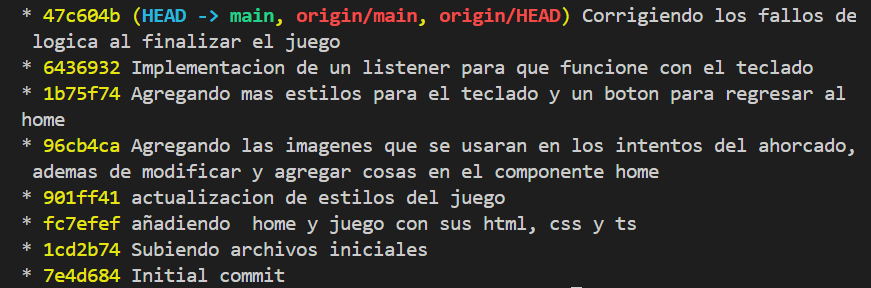
\includegraphics[width=1\textwidth]{img/commits.png}
                \caption{Imagen de los commits realizads en el repositorio}
                \label{fig:modelo_bd}
            \end{figure}
            
\end{itemize}


	\section{Codigo fuente}
	
	\subsection{Componentes usados}
            \begin{itemize}
                \item En la estructura del proyecto, hay dos componentes principales: Game y Home.
                \item Cada componente tiene su propio conjunto de archivos que siguen este esquema:
                \begin{itemize}
                    \item Archivo CSS (\texttt{.css}): Define los estilos específicos del componente.
                    \item Archivo HTML (\texttt{.html}): Define la estructura y el contenido del componente.
                    \item Archivo de pruebas (\texttt{.spec.ts}): Define las pruebas unitarias para el componente.
                    \item Archivo TypeScript (\texttt{.ts}): Define la lógica del componente, incluyendo sus propiedades y métodos.
                \end{itemize}
                \item Esta organización permite mantener el código modular y separado, facilitando el mantenimiento y la escalabilidad del proyecto.
            \end{itemize}
            \begin{figure}[h]
                \centering
                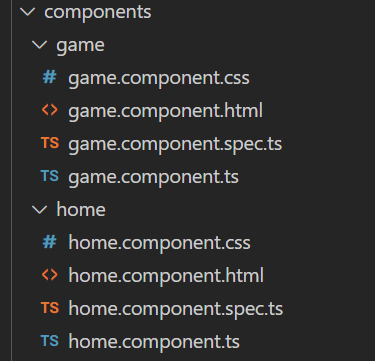
\includegraphics[width=0.5\textwidth]{img/components.png}
                \caption{Diagrama de la base de datos}
                \label{fig:modelo_bd}
            \end{figure}

  
\subsection{Componente Home}
\begin{itemize}
    \item El componente home se centra en la presentacion del juego, mostrando los nombres de los integrantes junto con las instrucciones del juego, ademas se añade un boton para pasar a la siguiente pestaña.
\end{itemize}

\begin{itemize}
    \item \textbf{HTML}:
    \begin{itemize}
        \item \textbf{Título Principal:} Un encabezado (\texttt{<h1>}) con el texto "Juego del ahorcado".
        \item \textbf{Descripción:} Un párrafo (\texttt{<p>}) que invita al usuario a poner a prueba sus habilidades de adivinanza.
        \item \textbf{Integrantes:} 
        \begin{itemize}
            \item Subtítulo (\texttt{<h2>}) con el texto "Integrantes".
            \item Lista (\texttt{<ul>}) que contiene los nombres de los miembros del equipo, cada uno en un elemento de lista (\texttt{<li>}) individual.
        \end{itemize}
        \item \textbf{Botón de Navegación:} Un botón (\texttt{<button>}) con el texto "Empezar a Jugar" que, al ser presionado, redirige al usuario a otra pestaña mediante la directiva \texttt{routerLink} de Angular.
        \item \textbf{Instrucciones:} 
        \begin{itemize}
            \item Subtítulo (\texttt{<h2>}) con el texto "Instrucciones".
            \item Lista (\texttt{<ul>}) que proporciona una guía paso a paso sobre cómo jugar el juego del ahorcado. Cada paso está contenido en un elemento de lista (\texttt{<li>}).
        \end{itemize}
    \end{itemize}
            \begin{figure}[h]
                \centering
                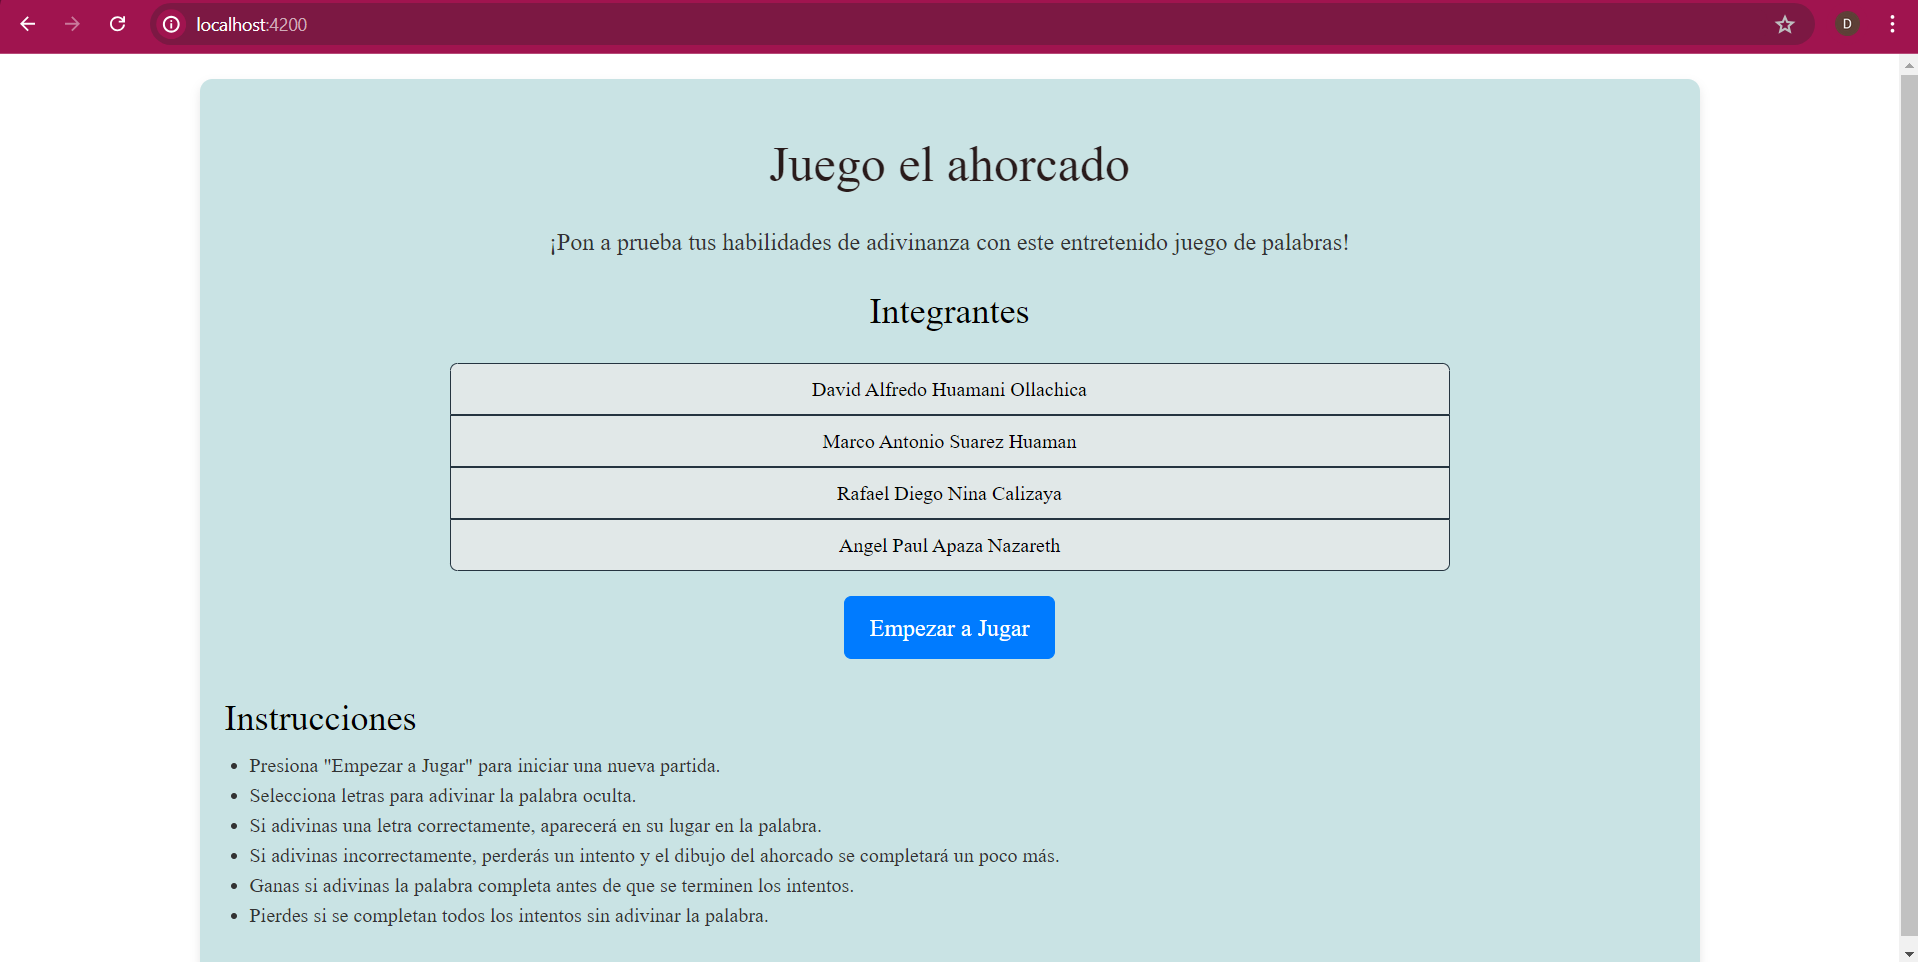
\includegraphics[width=1\textwidth]{img/home.png}
                \caption{Ejecucion de la pestaña home}
                \label{fig:modelo_bd}
            \end{figure}
    \begin{lstlisting}[language=html,caption={src\app\components\home\home.component.html}][H]
<div class="container">
    <h1 class="my-4">Juego el ahorcado </h1>
    <p class="mt-4">¡Pon a prueba tus habilidades de adivinanza con este entretenido juego de palabras!</p>
    <h2 class="my-4">Integrantes</h2>
    <ul class="list-group">
      <li class="list-group-item">David Alfredo Huamani Ollachica</li>
      <li class="list-group-item">Marco Antonio Suarez Huaman</li>
      <li class="list-group-item">Rafael Diego Nina Calizaya</li>
      <li class="list-group-item">Angel Paul Apaza Nazareth</li>
    </ul>
    <button routerLink="/game" class="btn btn-primary">Empezar a Jugar</button>
      <div class="instructions">
        <h2>Instrucciones</h2>
        <ul>
          <li>Presiona "Empezar a Jugar" para iniciar una nueva partida.</li>
          <li>Selecciona letras para adivinar la palabra oculta.</li>
          <li>Si adivinas una letra correctamente, aparecerá en su lugar en la palabra.</li>
          <li>Si adivinas incorrectamente, perderás un intento y el dibujo del ahorcado se completará un poco más.</li>
          <li>Ganas si adivinas la palabra completa antes de que se terminen los intentos.</li>
          <li>Pierdes si se completan todos los intentos sin adivinar la palabra.</li>
        </ul>
    </div>
</div>



    \end{lstlisting}


\subsection{Componente Game}

El componente \texttt{GameComponent} es una implementación de un juego del ahorcado utilizando Angular. A continuación se describe en detalle el código de este componente, incluyendo su lógica y estilos.

\subsubsection{Estructura del Componente}

    \begin{lstlisting}[language=js,caption ={src\app\components\game\game.component.ts}][H]
    import { Component, OnInit, HostListener } from '@angular/core';
import { Router } from '@angular/router';

@Component({
  selector: 'app-game',
  templateUrl: './game.component.html',
  styleUrls: ['./game.component.css']
})
export class GameComponent implements OnInit {
  alphabet: string[] = 'QWERTYUIOPASDFGHJKLÑZXCVBNM'.split('');
  words: string[] = ['ANGULAR', 'COMPONENTE', 'SERVICIO', 'DIRECTIVA', 'MODULO'];
  hiddenWord: string[] = [];
  incorrectLetters: string[] = [];
  remainingAttempts: number = 6;
  wins: number = 0;
  losses: number = 0;
  hangmanImage: string = '';
  showModal: boolean = false;
  modalMessage: string = '';

  private selectedWord: string = '';
  constructor(private router: Router) {}

  ngOnInit(): void {
    this.resetGame();
  }

  guessLetter(letter: string): void {
    if(this.gameEnd()){
      return;
    }
    if (this.selectedWord.includes(letter)) {
      for (let i = 0; i < this.selectedWord.length; i++) {
        if (this.selectedWord[i] === letter) {
          this.hiddenWord[i] = letter;
        }
      }
    } else {
      this.incorrectLetters.push(letter);
      this.remainingAttempts--;
    }
    
    this.updateHangmanImage();
    this.checkGameStatus();
  }

  isLetterGuessed(letter: string): boolean {
    return (this.hiddenWord.includes(letter) || this.incorrectLetters.includes(letter));
  }

  resetGame(): void {
    this.selectedWord = this.words[Math.floor(Math.random() * this.words.length)];
    this.hiddenWord = Array(this.selectedWord.length).fill('_');
    this.incorrectLetters = [];
    this.remainingAttempts = 6;
    this.updateHangmanImage();
  }

  updateHangmanImage(): void {
    this.hangmanImage = `assets/img${6 - this.remainingAttempts}.png`;
  }

  checkGameStatus(): void {
    if (this.hiddenWord.join('') === this.selectedWord) {
      this.wins++;
      this.showModalMessage('¡Ganaste!');
    } else if (this.remainingAttempts === 0) {
      this.losses++;
      this.showModalMessage('Perdiste. La palabra era ' + this.selectedWord);
    }
  }
  gameEnd(): boolean {
    return this.remainingAttempts === 0;
  }
  showModalMessage(message: string): void {
    this.modalMessage = message;
    this.showModal = true;
    setTimeout(() => {
      this.showModal = false;
    }, 3000);
  }
  navigateHome(){
    this.router.navigate(['/']);
  }

  @HostListener('window:keydown', ['$event'])
  handleKeyboardEvent(event: KeyboardEvent) {
    const letter = event.key.toUpperCase();
    if (!this.gameEnd() && this.alphabet.includes(letter) && !this.hiddenWord.includes(letter)) {
      this.guessLetter(letter);
    }
  }
}
\end{lstlisting}

\subsubsection{Explicación del Código}

\begin{itemize}
  \item \texttt{alphabet}: Array que contiene las letras del alfabeto.
  \item \texttt{words}: Array que contiene las palabras que se usarán en el juego.
  \item \texttt{hiddenWord}: Array que representa la palabra oculta con guiones bajos.
  \item \texttt{incorrectLetters}: Array que contiene las letras incorrectas adivinadas por el jugador.
  \item \texttt{remainingAttempts}: Número de intentos restantes antes de perder el juego.
  \item \texttt{wins}: Contador de juegos ganados.
  \item \texttt{losses}: Contador de juegos perdidos.
  \item \texttt{hangmanImage}: Ruta de la imagen del ahorcado.
  \item \texttt{showModal}: Booleano que controla la visibilidad del modal de mensajes.
  \item \texttt{modalMessage}: Mensaje a mostrar en el modal.
  \item \texttt{selectedWord}: Palabra seleccionada para el juego actual.
\end{itemize}

\subsubsection{Métodos}

\begin{itemize}
  \item \texttt{ngOnInit}: Inicializa el juego llamando a \texttt{resetGame}.
  \item \texttt{guessLetter}: Maneja la lógica de adivinar una letra.
  \item \texttt{isLetterGuessed}: Verifica si una letra ya ha sido adivinada.
  \item \texttt{resetGame}: Reinicia el juego con una nueva palabra.
  \item \texttt{updateHangmanImage}: Actualiza la imagen del ahorcado basada en los intentos restantes.
  \item \texttt{checkGameStatus}: Verifica el estado del juego (ganado o perdido).
  \item \texttt{gameEnd}: Verifica si el juego ha terminado.
  \item \texttt{showModalMessage}: Muestra un mensaje en un modal.
  \item \texttt{navigateHome}: Navega a la página de inicio.
  \item \texttt{handleKeyboardEvent}: Maneja eventos de teclado para adivinar letras.
\end{itemize}

\subsubsection{HTML del Componente}

\begin{lstlisting}[language=html,caption ={src\app\components\game\game.component.html}][H]
<div class="container">
  <div class="game-header">
    <h1>Juego del Ahorcado</h1>
    <p>Encuentra la palabra:</p>
    <div class="word">
      <span *ngFor="let char of hiddenWord">{{ char }}</span>
    </div>
  </div>

  <button class="btn-exit"  (click)="navigateHome()">
    Regresar al inicio
  </button>
  <div class="game-body">
    <img [src]="hangmanImage" alt="Hangman" class="hangman-image">
    <p>Intentos restantes: {{ remainingAttempts }}</p>
    <p>Letras incorrectas: {{ incorrectLetters.join(', ') }}</p>
    <div class="keycontainer">
      <div class="letters">
        <button class="letter btn" *ngFor="let letter of alphabet" (click)="guessLetter(letter)" [disabled]="isLetterGuessed(letter)">
            <div class="tecla caracter">
                {{ letter }}
            </div>
        </button>
      </div>
    </div>
  </div>
  
  <div class="game-footer">
    <p class="win-counter">Ganaste: {{ wins }}</p>
    <p class="lose-counter">Perdiste: {{ losses }}</p>
    <button (click)="resetGame()" class="btn btn-primary">Jugar de nuevo</button>
  </div>
  
  <div class="modal" [ngClass]="{'show': showModal}" role="dialog" aria-hidden="true">
    <div class="modal-dialog" role="document">
      <div class="modal-content">
        <div class="modal-header">
          <h5 class="modal-title">{{ modalMessage }}</h5>
        </div>
      </div>
    </div>
  </div>
</div>
\end{lstlisting}

\subsubsection{CSS del Componente}

\begin{lstlisting}[language=css,caption ={src\app\components\game\game.component.css}][H]
@import url('https://fonts.googleapis.com/css2?family=Baskervville+SC&display=swap');

.container {
    text-align: center;
    margin-top: 20px;
    position: relative;
    font-family: 'Arial', sans-serif;
    background: linear-gradient(to right, #f80707 0%, #38fa0c 100%);
    padding: 20px;
    border-radius: 15px;
    box-shadow: 0 4px 10px rgba(0, 0, 0, 0.2);
    animation: fadeIn 1s ease-in-out;
  }
  
  @keyframes fadeIn {
    from {
      opacity: 0;
      transform: translateY(-20px);
    }
    to {
      opacity: 1;
      transform: translateY(0);
    }
  }
  
  .word {
    font-size: 32px;
    margin-bottom: 40px;
    letter-spacing: 10px;
    font-weight: bold;
    color: #4a4a4a;
    text-shadow: 1px 1px 2px rgba(0, 0, 0, 0.1);
    background: rgba(89, 249, 9, 0.8);
    padding: 10px 20px;
    border-radius: 10px;
    display: inline-block;
  }
  
  .hangman-image {
    width: 200px;
    height: auto;
    margin-bottom: 20px;
    transition: transform 0.3s ease, box-shadow 0.3s ease;
    border-radius: 10px;
    box-shadow: 0 4px 10px rgba(0, 0, 0, 0.2);
  }
  
  .hangman-image:hover {
    transform: scale(1.1);
    box-shadow: 0 6px 15px rgba(0, 0, 0, 0.3);
  }
  .keycontainer{
    display: flex;
    align-items: center;
    justify-content: center;
    max-width: 700px;
    margin: 0 auto; 
  }
  .letters{
    display: flex;
    gap: 20px;
    flex-wrap: wrap;
    margin: auto;
    max-width: 100%;
    justify-content: center;

  }
  .letters button {
    font-family: "Baskervville SC", serif;
    font-weight: 400;
    font-style: normal;
    font-size: 1rem;
    background-color: beige;
    color: #4A4A4A;
    border: 1px black solid;
    box-shadow: 5px 5px #4A4A4A;
    border-radius: 1rem;
    min-width: 50px;
    max-width: 50px;
    min-height: 50px;
    max-height: 50px;
    cursor: pointer; 
    transition: transform 0.3s ease, color 0.3s ease, background-color 0.3s ease;
  }
  
  .letters button:hover {
    background-color: #4A4A4A;
    color: beige;
    transform: scale(1.2); 
  }
  
  .letters button:disabled {
    background-color: #ccc;
    color: #999;
    cursor: not-allowed;
    transform: scale(1);
    box-shadow: none;
  }
  
  .game-footer {
    margin-top: 20px;
    display: flex;
    justify-content: center;
    gap: 20px;
  }
  
  .win-counter {
    position: absolute;
    top: 10px;
    left: 10px;
    color: green;
    font-weight: bold;
    font-size: 18px;
    background: rgba(255, 255, 255, 0.8);
    padding: 5px 10px;
    border-radius: 5px;
  }
  
  .lose-counter {
    position: absolute;
    top: 10px;
    right: 10px;
    color: red;
    font-weight: bold;
    font-size: 18px;
    background: rgba(255, 255, 255, 0.8);
    padding: 5px 10px;
    border-radius: 5px;
  }
  
  .modal {
    display: none;
    position: fixed;
    top: 0;
    left: 0;
    width: 100%;
    height: 100%;
    background-color: rgba(0, 0, 0, 0.5);
    align-items: center;
    justify-content: center;
    z-index: 9999;
    animation: fadeInModal 0.5s ease forwards;
  }
  
  .modal.show {
    display: flex;
  }
  
  @keyframes fadeInModal {
    from {
      opacity: 0;
    }
    to {
      opacity: 1;
    }
  }
  
  .modal-dialog {
    background-color: white;
    padding: 20px;
    border-radius: 10px;
    box-shadow: 0 4px 8px rgba(0, 0, 0, 0.2);
    animation: slideInModal 0.5s ease forwards, swing 2s infinite;
  }
  
  @keyframes slideInModal {
    from {
      transform: translateY(-50%);
      opacity: 0;
    }
    to {
      transform: translateY(0);
      opacity: 1;
    }
  }
  
  @keyframes swing {
    20% {
      transform: rotate(15deg);
    }
    40% {
      transform: rotate(-10deg);
    }
    60% {
      transform: rotate(5deg);
    }
    80% {
      transform: rotate(-5deg);
    }
    100% {
      transform: rotate(0deg);
    }
  }
  
  .btn {
    padding: 10px 20px;
    font-size: 16px;
    border: none;
    border-radius: 5px;
    background-color: #007bff;
    color: #fff;
    cursor: pointer;
    transition: background-color 0.3s ease, transform 0.3s ease, box-shadow 0.3s ease;
    box-shadow: 0 2px 5px rgba(0, 0, 0, 0.1);

  }
  
  .btn:hover {
    background-color: #0056b3;
    transform: scale(1.05);
    box-shadow: 0 4px 10px rgba(0, 0, 0, 0.2);
  }
  
  @media (max-width: 600px) {
    .letters button {
      font-size: 16px;
      padding: 8px 12px;
    }
  
    .word {
      font-size: 24px;
    }
  
    .btn {
      font-size: 14px;
      padding: 8px 16px;
    }
  }
  
  .btn-exit {
    position: fixed;
    top: var(--button-top-position);
    left: 5px;
    background-color: #ff4c4c;
    color: white;
    border: none;
    border-radius: 5px;
    cursor: pointer;
    box-shadow: 0 4px 6px rgba(0, 0, 0, 0.1);
    font-size: 16px;
    transition: all 0.3s ease-in-out;
  }
  
.btn-exit:hover {
    background-color: #ff1a1a;
    box-shadow: 0 6px 8px rgba(0, 0, 0, 0.2);
    transform: scale(1.1);
}

.btn-exit:active {
    background-color: #e60000;
    box-shadow: 0 2px 4px rgba(0, 0, 0, 0.2);
    transform: scale(0.9);
}

@keyframes fadeIn {
    0% {
        opacity: 0;
        transform: translateY(-20px);
    }
    100% {
        opacity: 1;
        transform: translateY(0);
    }
}

.btn-exit {
    animation: fadeIn 0.8s ease-out;
}

@keyframes pulse {
    0% {
        box-shadow: 0 0 0 0 rgba(255, 76, 76, 0.7);
    }
    70% {
        box-shadow: 0 0 0 20px rgba(255, 76, 76, 0);
    }
    100% {
        box-shadow: 0 0 0 0 rgba(255, 76, 76, 0);
    }
}

.btn-exit {
    animation: pulse 1.5s infinite;
}
\end{lstlisting}

\subsubsection{Explicación de los Estilos}

\begin{itemize}
  \item \texttt{.container}: Estilos para el contenedor principal, incluyendo fuente, colores de fondo y animación de entrada.
  \item \texttt{.word}: Estilos para la palabra oculta, con espaciado entre letras y efectos de sombra.
  \item \texttt{.hangman-image}: Estilos para la imagen del ahorcado, incluyendo tamaño, transición y efectos de hover.
  \item \texttt{.keycontainer}: Estilos para el contenedor de teclas.
  \item \texttt{.letters}: Estilos para las letras del teclado virtual, con efectos de hover y deshabilitado.
  \item \texttt{.game-footer}: Estilos para el pie de página del juego.
  \item \texttt{.win-counter} y \texttt{.lose-counter}: Estilos para los contadores de victorias y derrotas.
  \item \texttt{.modal}: Estilos para el modal, incluyendo animaciones de entrada.
  \item \texttt{.btn}: Estilos para los botones, con efectos de hover y transiciones.
  \item \texttt{.btn-exit}: Estilos para el botón de salida, con animaciones de entrada y efectos de pulsación.
\end{itemize}

Este componente implementa todas las funcionalidades necesarias para jugar al ahorcado, manejando eventos de teclado, actualizando la interfaz de usuario y mostrando mensajes de victoria o derrota de manera efectiva.



\begin{figure}[h]
    \centering
    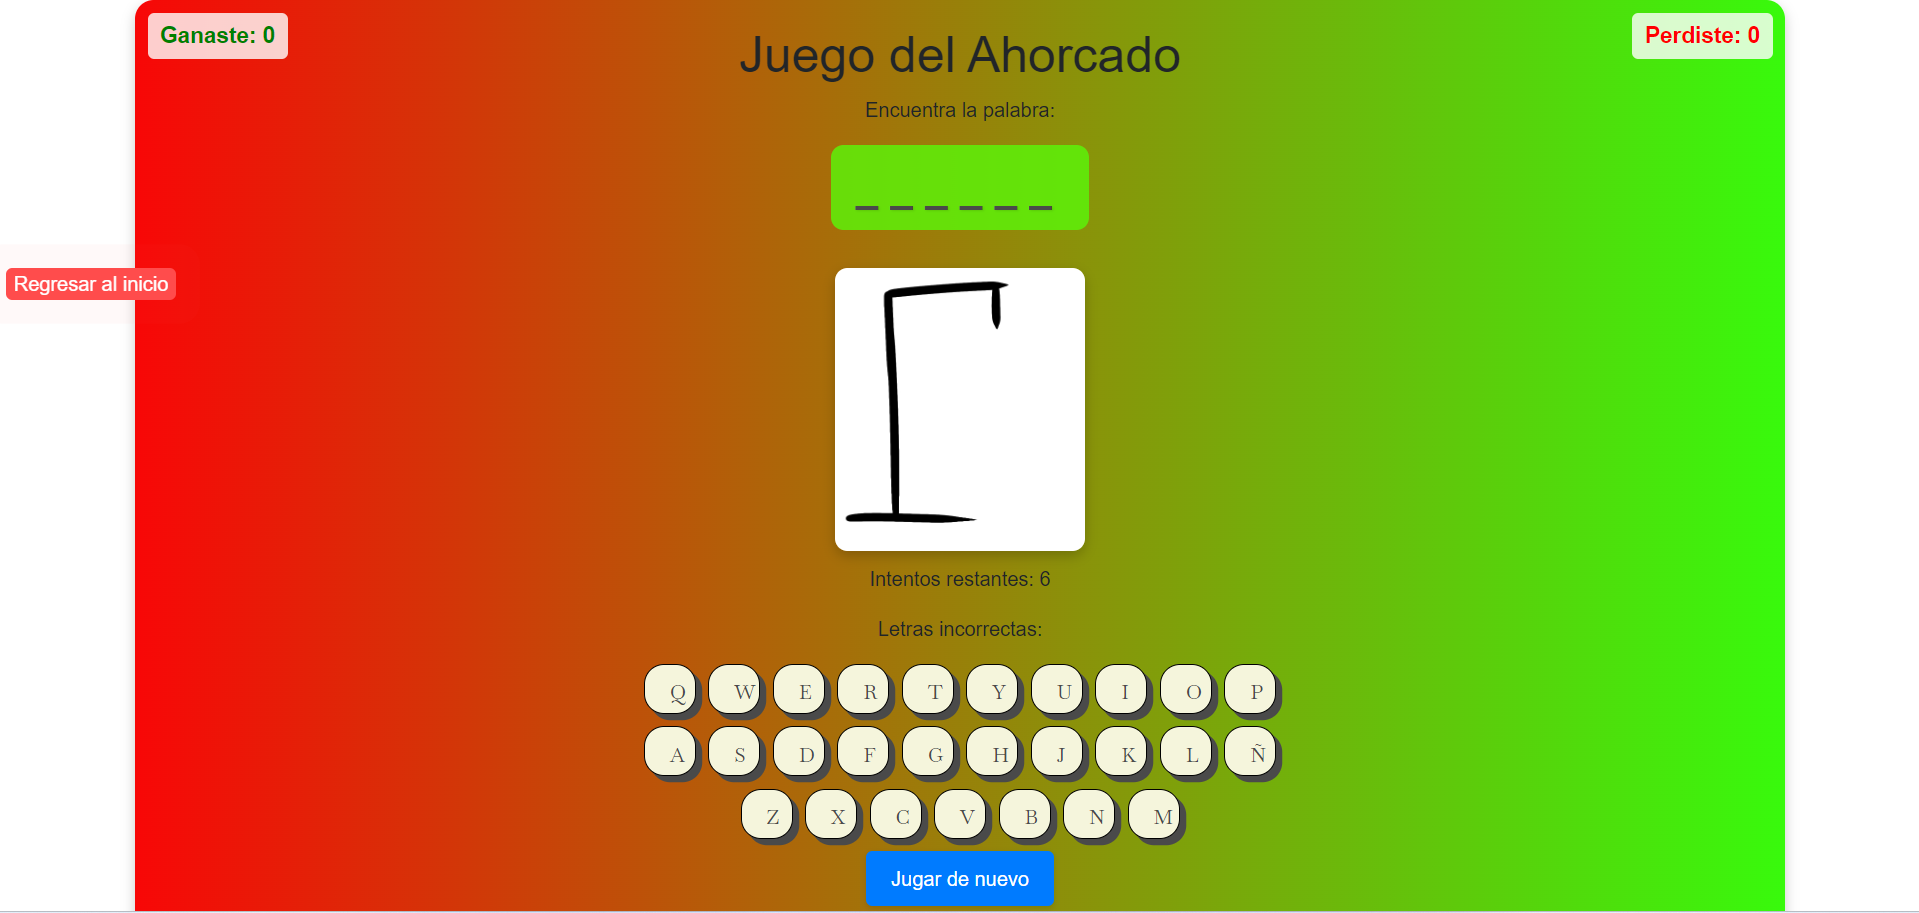
\includegraphics[width=1\textwidth]{img/game1.png}
    \caption{Ejecución del juego 1}
    \label{fig:game1}
\end{figure}

\begin{figure}[h]
    \centering
    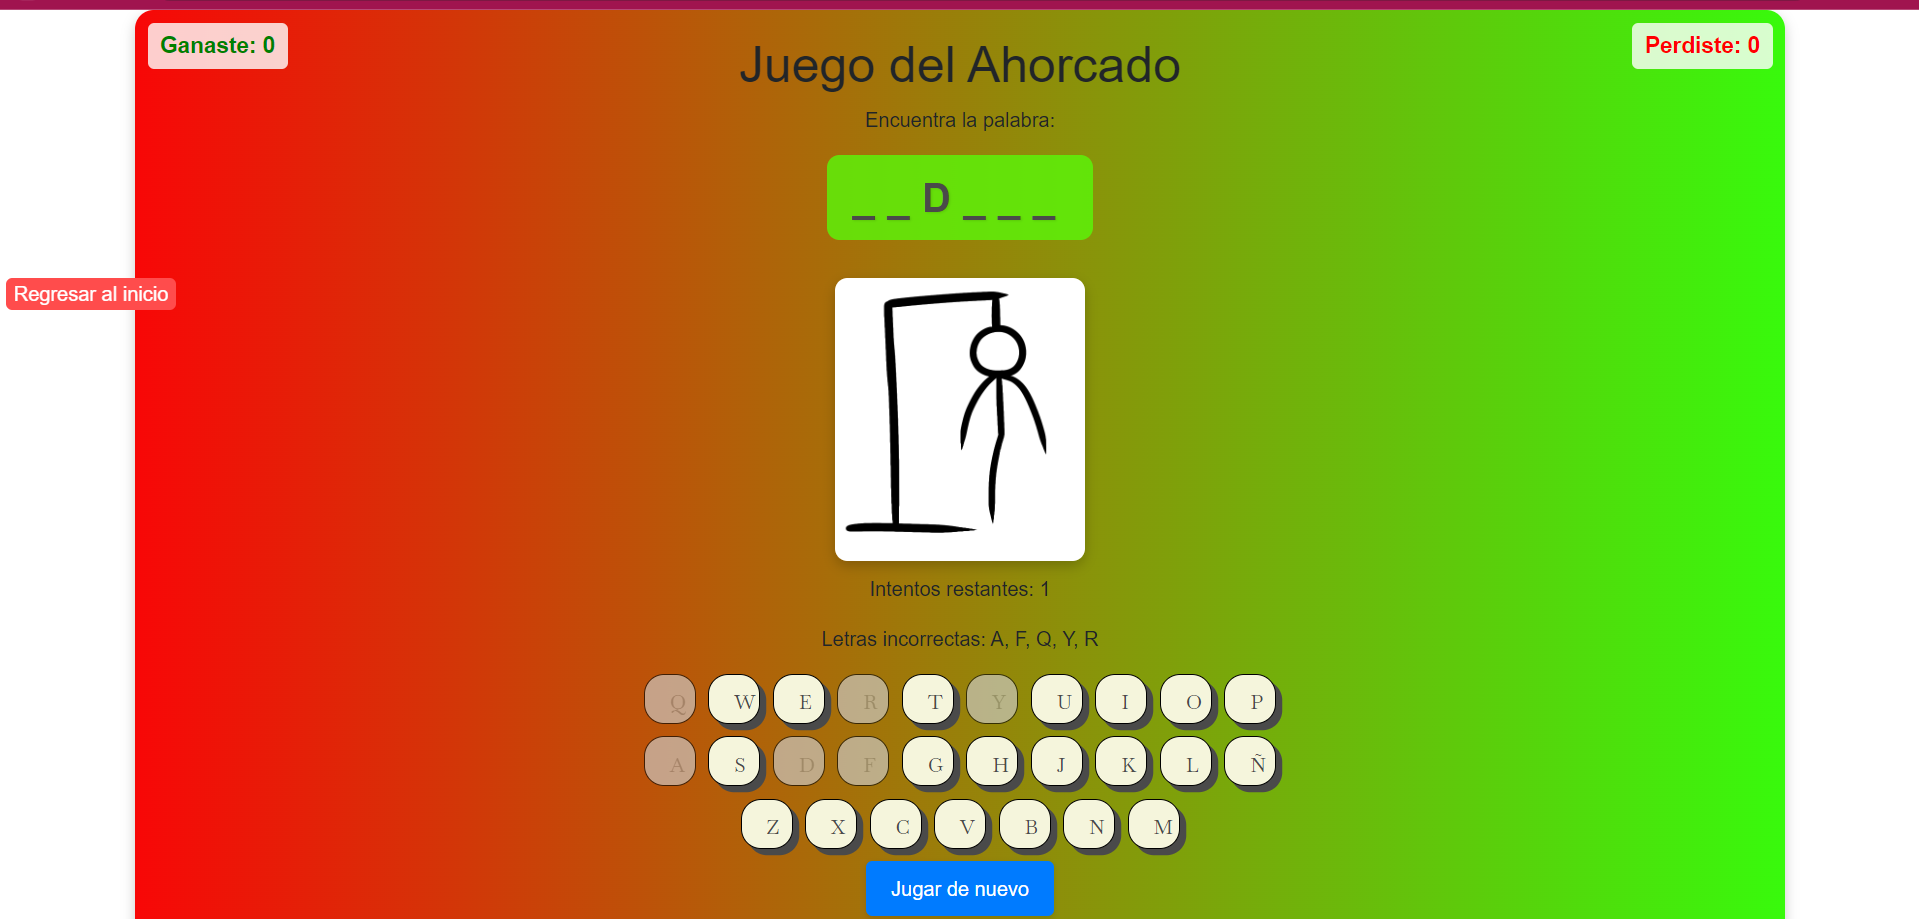
\includegraphics[width=1.2\textwidth]{img/game2.png}
    \caption{Ejecución del juego 2}
    \label{fig:game2}
\end{figure}

\begin{figure}[h]
    \centering
    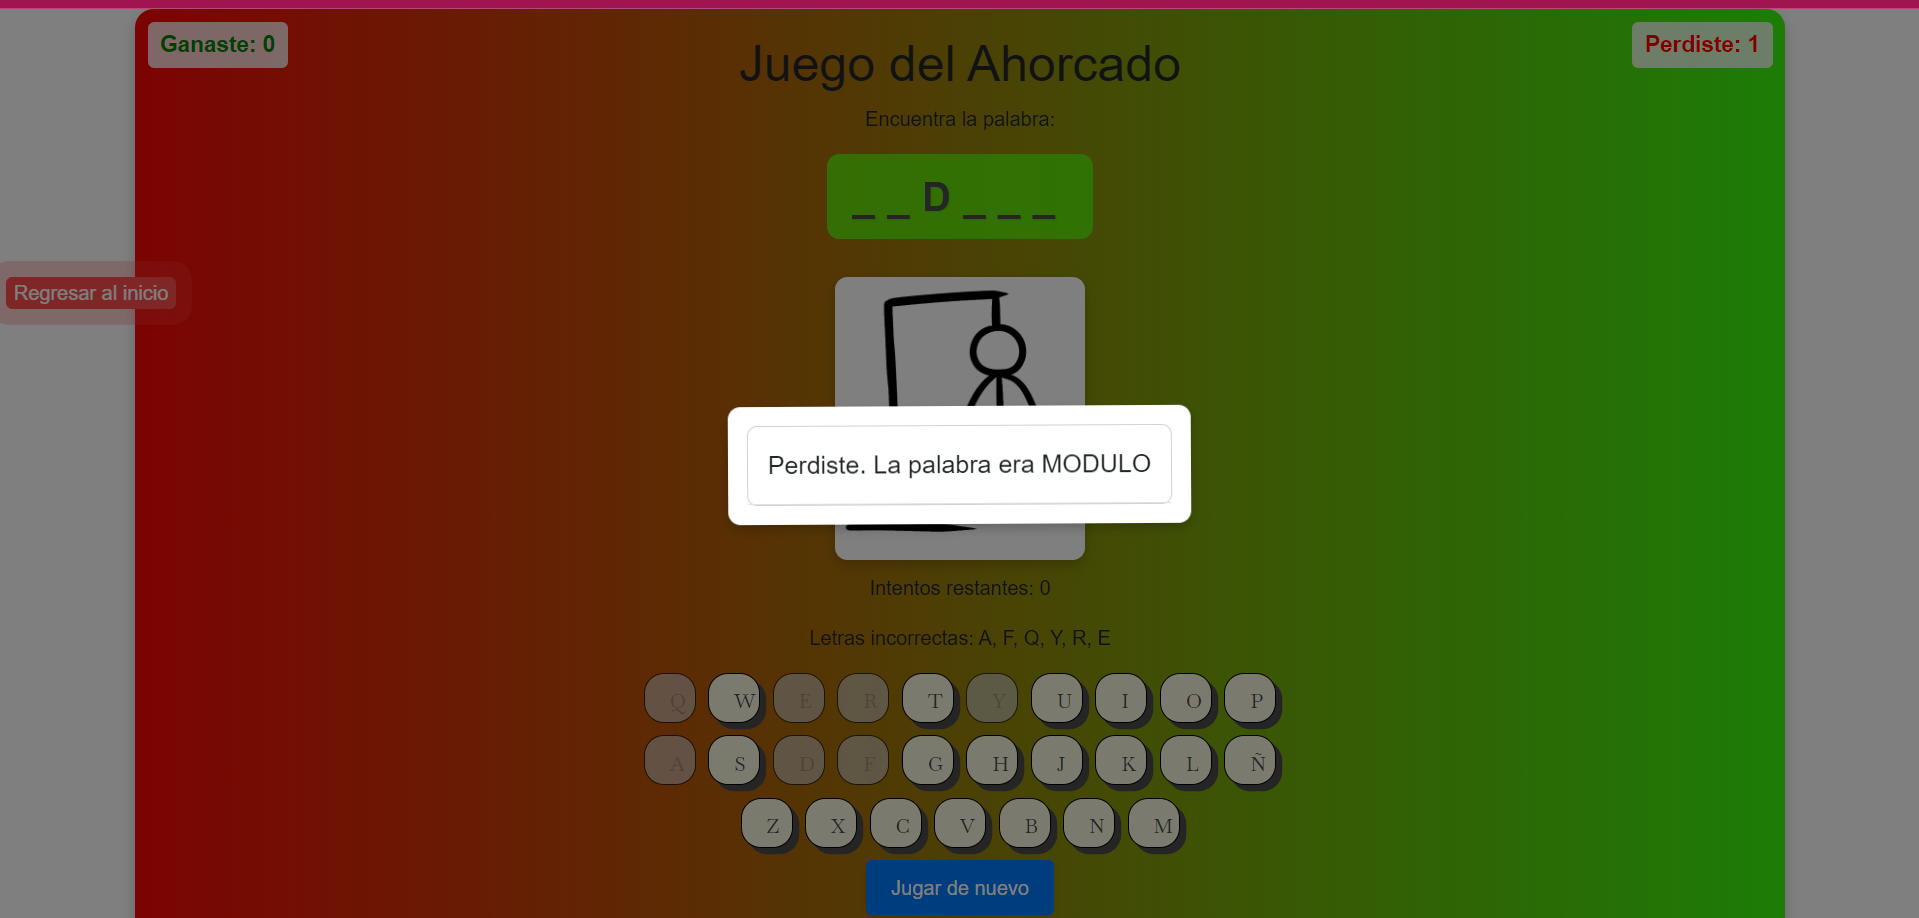
\includegraphics[width=1\textwidth]{img/game3.png}
    \caption{Ejecución del juego 3}
    \label{fig:game3}
\end{figure}

\begin{figure}[h]
    \centering
    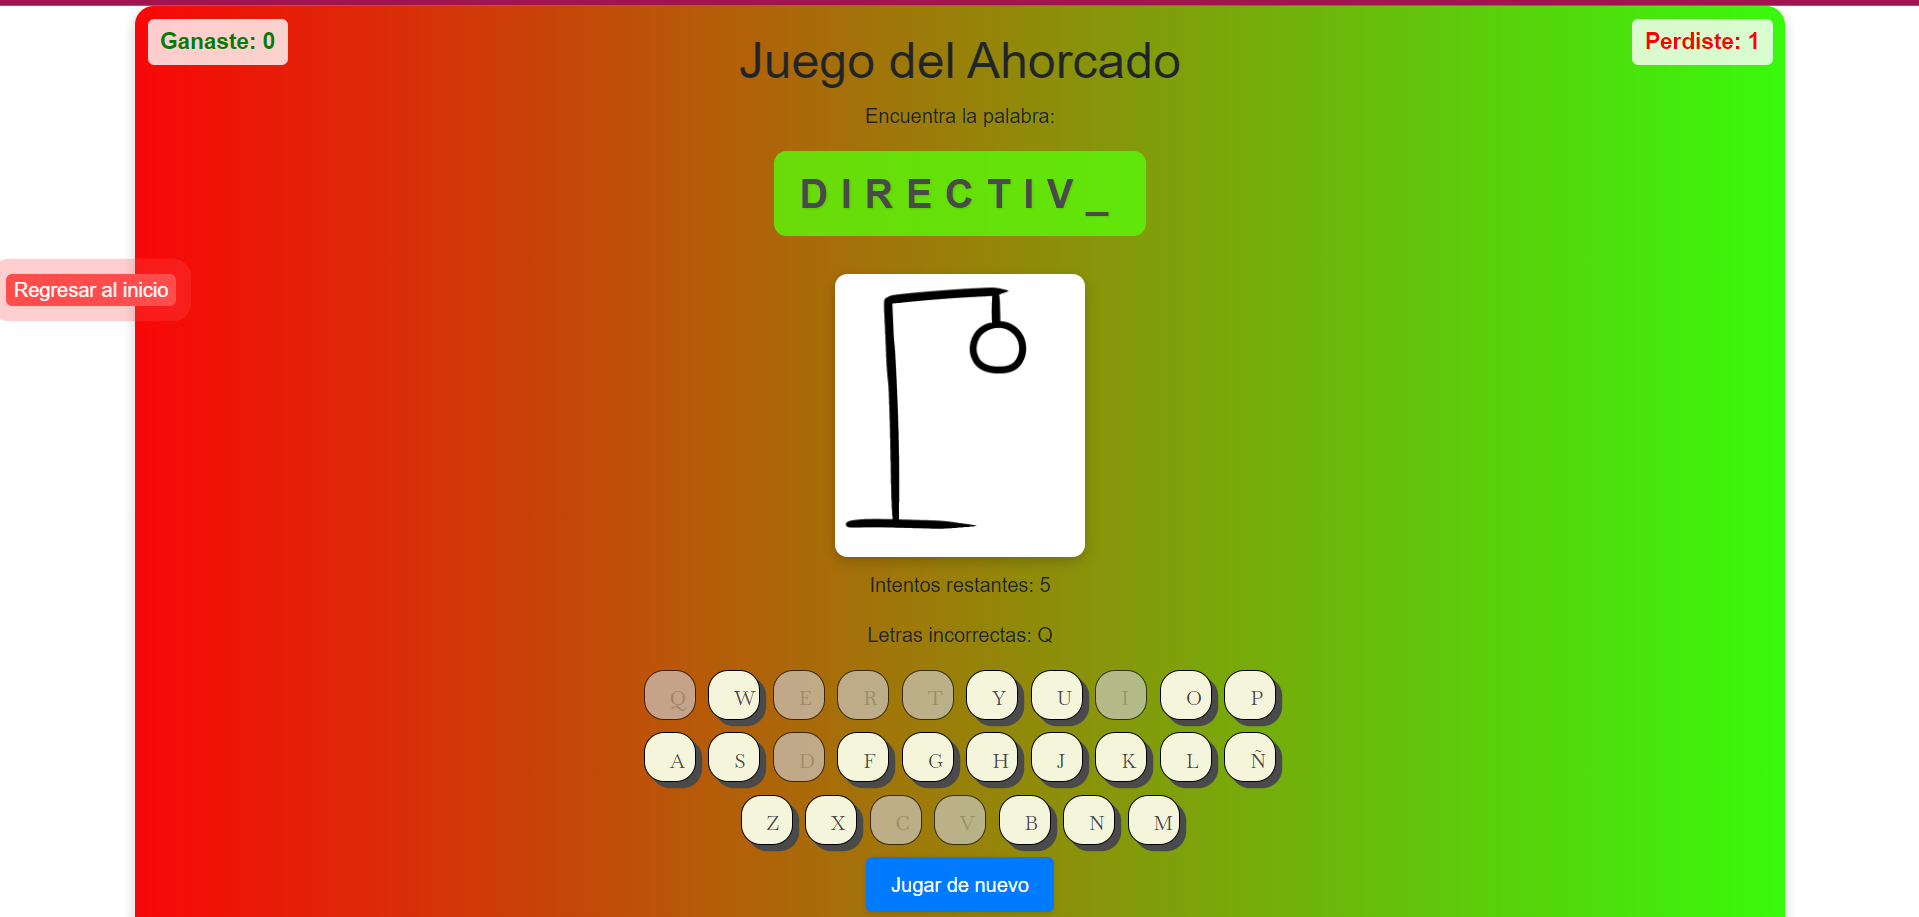
\includegraphics[width=1\textwidth]{img/game4.png}
    \caption{Ejecución del juego 4}
    \label{fig:game4}
\end{figure}

\begin{figure}[h]
    \centering
    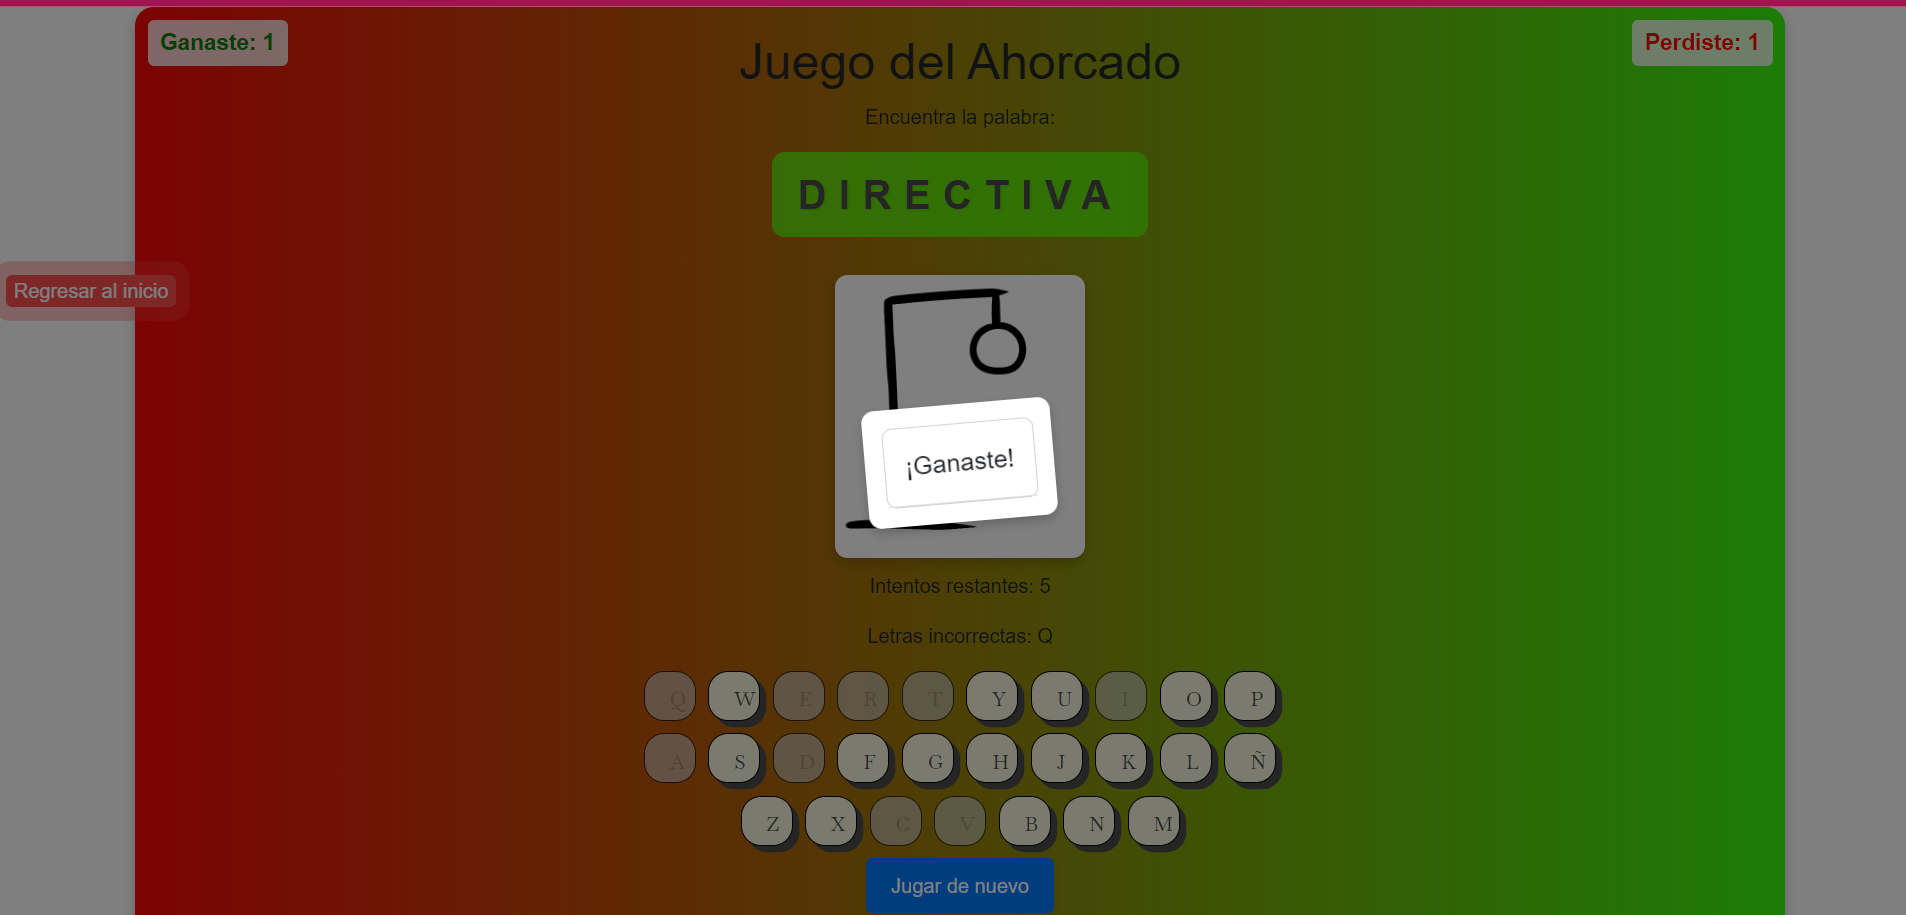
\includegraphics[width=1\textwidth]{img/game5.png}
    \caption{Ejecución del juego 5}
    \label{fig:game5}
\end{figure}


    
    



	\section{\textcolor{red}{Rúbricas}}
	
	\subsection{\textcolor{red}{Sobre el informe}}
	\begin{table}[H]
		\caption{Tipo de Informe}
		\setlength{\tabcolsep}{0.5em} % for the horizontal padding
		{\renewcommand{\arraystretch}{1.5}% for the vertical padding
		\begin{tabular}{|p{3cm}|p{12cm}|}
			\hline
			\multicolumn{2}{|c|}{\textbf{\textcolor{red}{Informe}}}  \\
			\hline 
			\textbf{\textcolor{red}{Latex}} & \textcolor{blue}{El informe está en formato PDF desde Latex,  con un formato limpio (buena presentación) y facil de leer.}   \\ 
			\hline 
			
			
		\end{tabular}
	}
	\end{table}
	
	\clearpage

	\subsection{\textcolor{red}{Rúbrica para el contenido del Informe y demostración}}
	\begin{itemize}			
		\item El alumno debe marcar o dejar en blanco en celdas de la columna \textbf{Checklist} si cumplio con el ítem correspondiente.
		\item Si un alumno supera la fecha de entrega,  su calificación será sobre la nota mínima aprobada, siempre y cuando cumpla con todos lo items.
		\item El alumno debe autocalificarse en la columna \textbf{Estudiante} de acuerdo a la siguiente tabla:
	
		\begin{table}[ht]
			\caption{Niveles de desempeño}
			\begin{center}
			\begin{tabular}{ccccc}
    			\hline
    			 & \multicolumn{4}{c}{Nivel}\\
    			\cline{1-5}
    			\textbf{Puntos} & Insatisfactorio 25\%& En Proceso 50\% & Satisfactorio 75\% & Sobresaliente 100\%\\
    			\textbf{2.0}&0.5&1.0&1.5&2.0\\
    			\textbf{4.0}&1.0&2.0&3.0&4.0\\
    		\hline
			\end{tabular}
		\end{center}
	\end{table}	
	
	\end{itemize}
	
	\begin{table}[H]
		\caption{Rúbrica para contenido del Informe y demostración}
		\setlength{\tabcolsep}{0.5em} % for the horizontal padding
		{\renewcommand{\arraystretch}{1.5}% for the vertical padding
		%\begin{center}
		\begin{tabular}{|p{2.7cm}|p{7cm}|x{1.3cm}|p{1.2cm}|p{1.5cm}|p{1.1cm}|}
			\hline
    		\multicolumn{2}{|c|}{Contenido y demostración} & Puntos & Checklist & Estudiante & Profesor\\
			\hline
			\textbf{1. GitHub} & Hay enlace URL activo del directorio para el  laboratorio hacia su repositorio GitHub con código fuente terminado y fácil de revisar. &2 &X &2 & \\ 
			\hline
			\textbf{2. Commits} &  Hay capturas de pantalla de los commits más importantes con sus explicaciones detalladas. (El profesor puede preguntar para refrendar calificación). &4 &X &4 & \\ 
			\hline 
			\textbf{3. Código fuente} &  Hay porciones de código fuente importantes con numeración y explicaciones detalladas de sus funciones. &2 &X &2 & \\ 
			\hline 
			\textbf{4. Ejecución} & Se incluyen ejecuciones/pruebas del código fuente  explicadas gradualmente. &2 &X &2 & \\ 
			\hline			
			\textbf{5. Pregunta} & Se responde con completitud a la pregunta formulada en la tarea.  (El profesor puede preguntar para refrendar calificación).  &2 &X &2 & \\ 
			\hline	
			\textbf{6. Fechas} & Las fechas de modificación del código fuente estan dentro de los plazos de fecha de entrega establecidos. &2 &X &2 & \\ 
			\hline 
			\textbf{7. Ortografía} & El documento no muestra errores ortográficos. &2 &X &2 & \\ 
			\hline 
			\textbf{8. Madurez} & El Informe muestra de manera general una evolución de la madurez del código fuente,  explicaciones puntuales pero precisas y un acabado impecable.   (El profesor puede preguntar para refrendar calificación).  &4 &X &3 & \\ 
			\hline
			\multicolumn{2}{|c|}{\textbf{Total}} &20 & &19 & \\ 
			\hline
		\end{tabular}
		%\end{center}
		%\label{tab:multicol}
		}
	\end{table}
	
\clearpage

\section{Referencias}
\begin{itemize}			
	\item \url{https://angular.dev/}
	\item \url{https://docs.angular.lat/}


\end{itemize}	
	
%\clearpage
%\bibliographystyle{apalike}
%\bibliographystyle{IEEEtranN}
%\bibliography{bibliography}
			
\end{document}
